\label{5_resultados}

\section{Parâmetros analisados}

Como um AG trabalha com tentativa-e-erro, não há uma geração exata para a qual pode ser prevista uma determinada solução (ou proximidade à solução). Para se analisar a evolução dos indivíduos ao longo das gerações, este trabalho focou em analisar os seguintes parâmetros:

\begin{itemize}
	\item Valor mínimo de fitness em um indivíduo;
	\item Valor máximo de fitness em um indivíduo;
	\item Valor médio de fitness entre todos os indivíduos;
	\item Desvio padrão dos valores de fitness.
\end{itemize}

O desvio padrão utilizado aqui foi o amostral, dado por:

\begin{equation}
	\sigma = \sqrt{\frac{1}{N-1} \sum_{i=1}^N (x_i - \overline{x})^2}
\end{equation}

Os gráficos criados tiveram como base uma única simulação do AG para o problema e parâmetros de entrada escolhidos.

Como já foi comentado antes, se não for mencionado o contrário (mesmo para o caso adaptativo), utilizou-se 0.9 para $p_c$ e 0.01 para $p_m$. Todas as execuções utilizaram 100 indivíduos, 200 gerações e elitismo do melhor indivíduo. Se um problema convergiu completamente para a melhor solução antes das 200 gerações completarem, os gráficos foram reduzidos para melhor visualização, uma vez que os pontos extras não trariam novas informações para nós.

As simulações feitas com uso do AGA foram utilizadas para comparação com a implementação estática do AG. Além disso, foi avaliado o comportamento adaptativo de $p_m$ ao longo das gerações.

\section{OneMax Booleano}

\subsection{Caso Estático}

Este problema foi considerado simples de ser resolvido por um AG, uma vez que poucas mutações em um gene já fariam com que ele trouxesse o valor máximo. As figuras \ref{fig:onemax_boolean} e \ref{fig:onemax_boolean_std} demonstram exatamente isso, com convergência completa dos indivíduos para a solução ótima após 93 gerações.

\begin{figure}[ht!]
    \centering 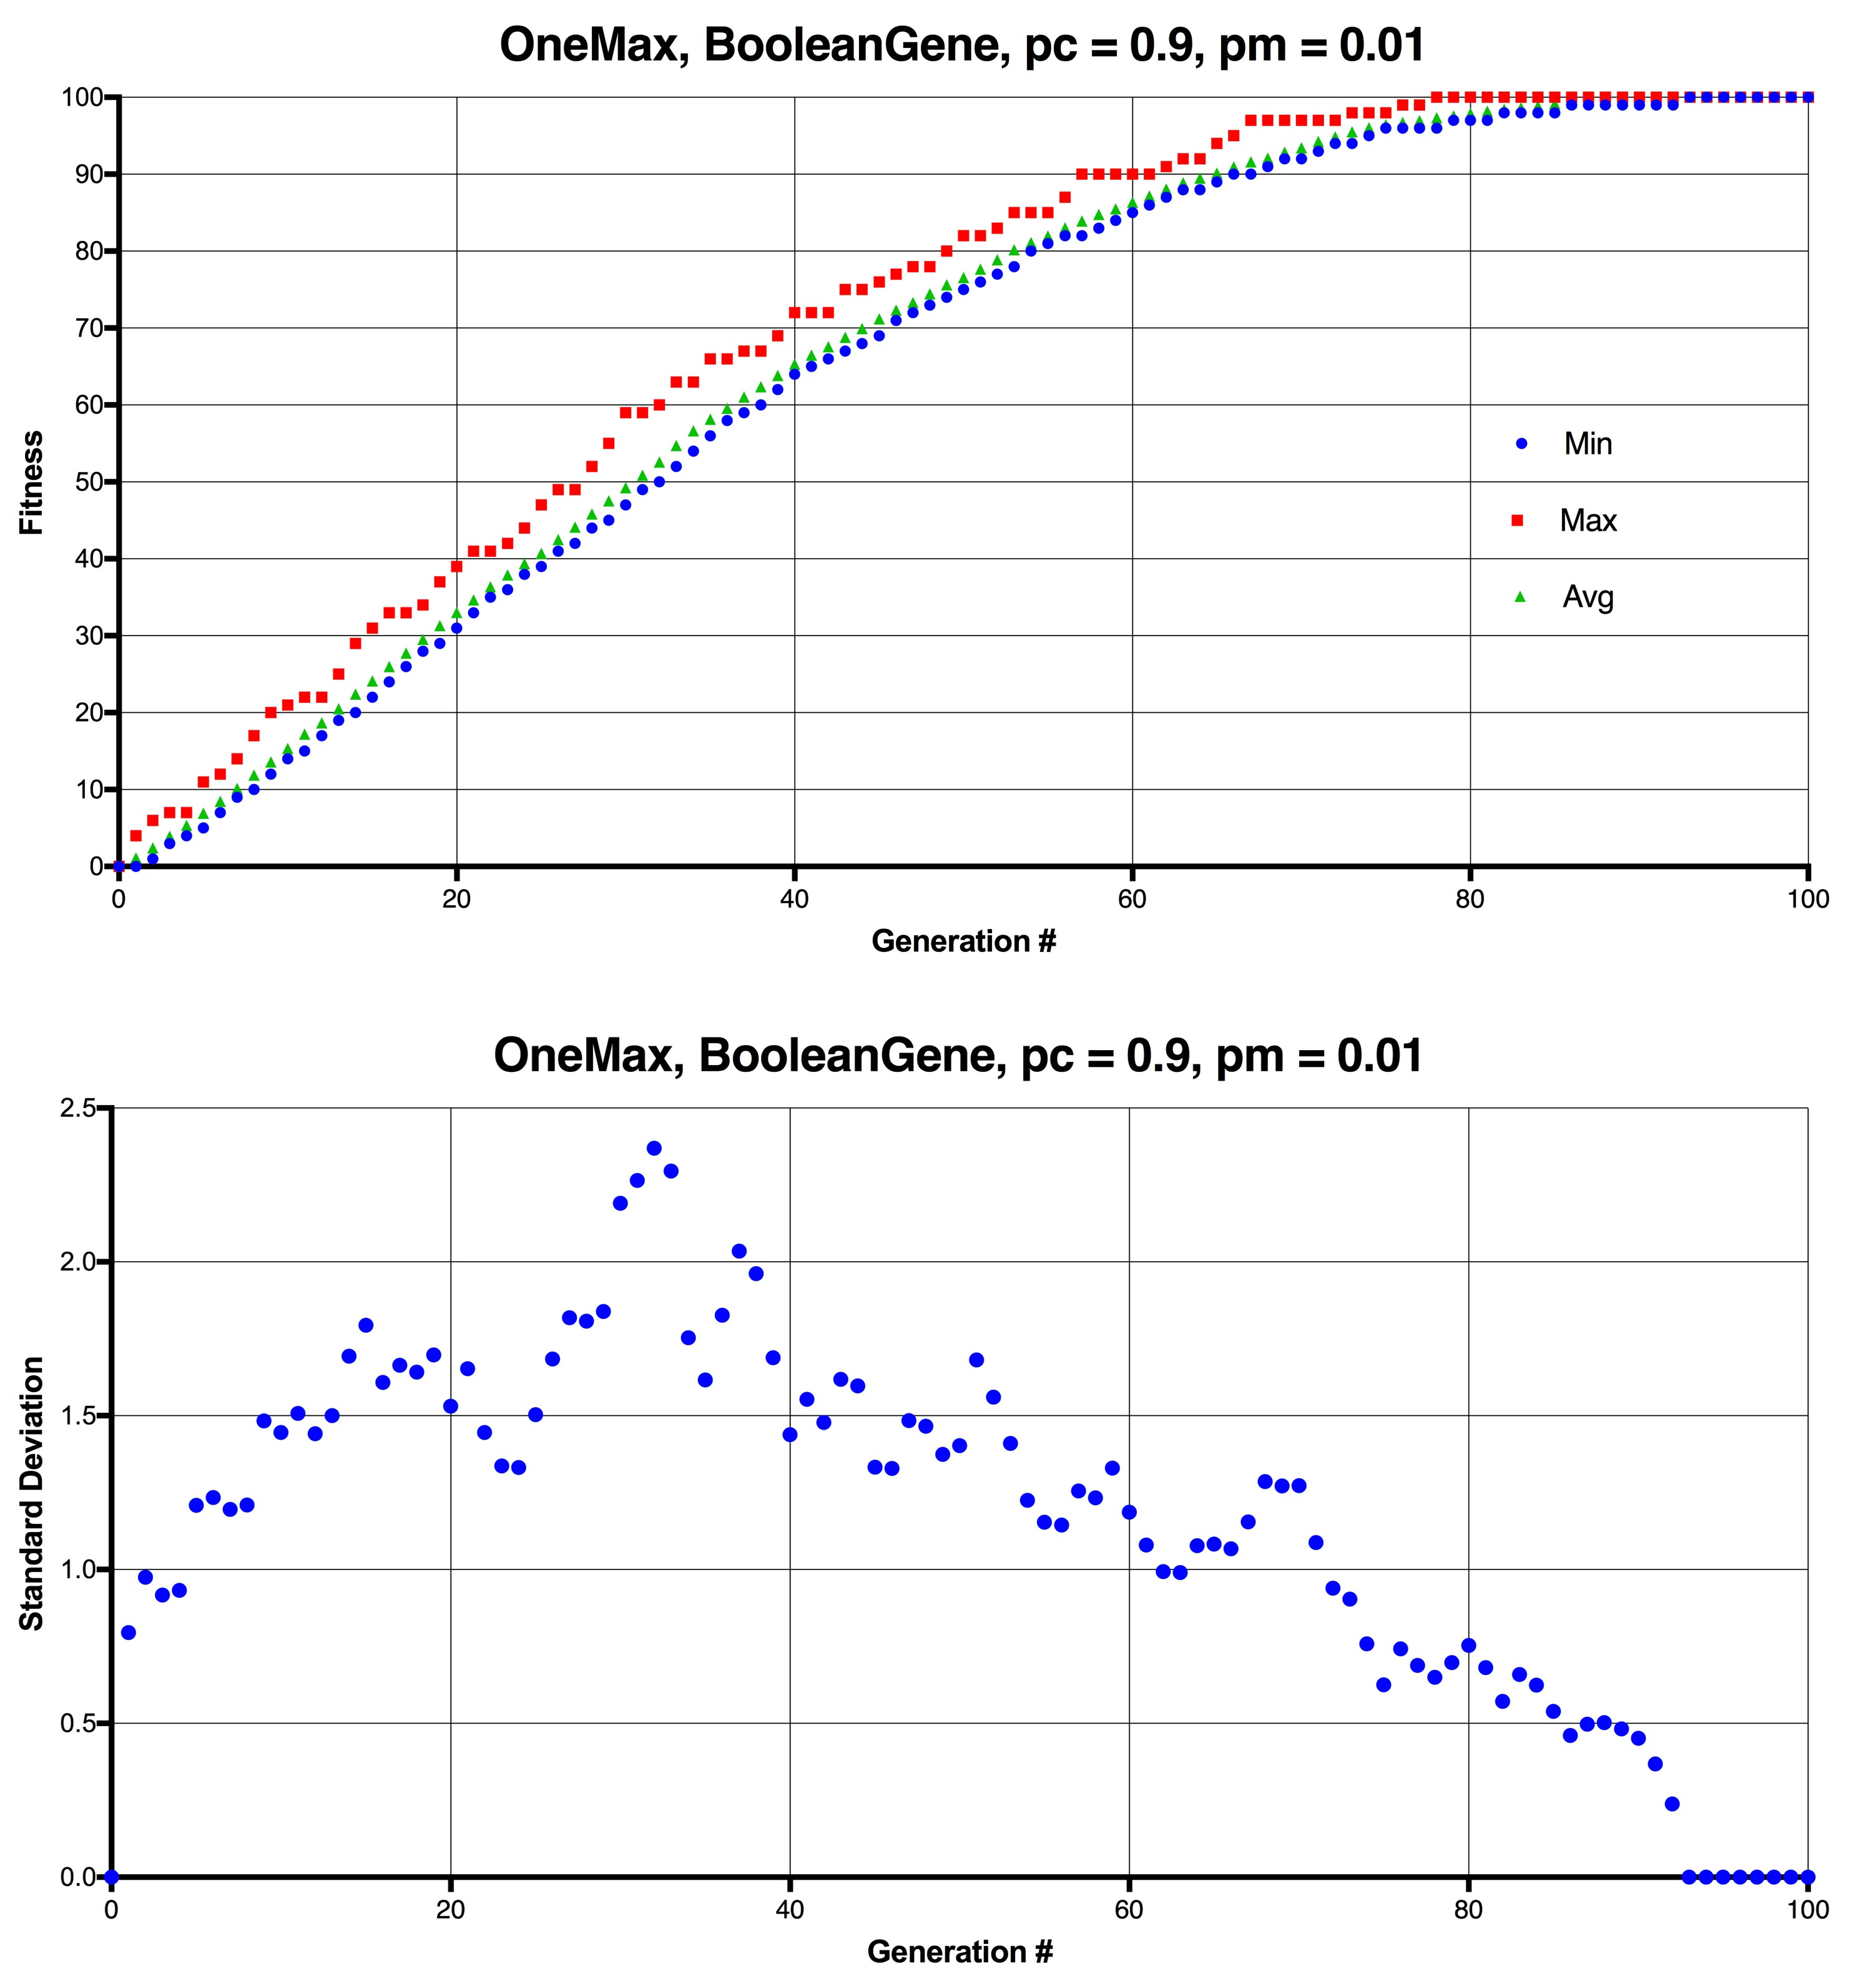
\includegraphics[width=1.0\textwidth]{onemax_boolean.jpg}
    \caption{Evolução do fitness para o problema do OneMax Booleano mostrando mínimo, máximo e valor médio ($p_c=0.9$, $p_m=0.01$).}
    \label{fig:onemax_boolean}
\end{figure}

\begin{figure}[ht!]
    \centering 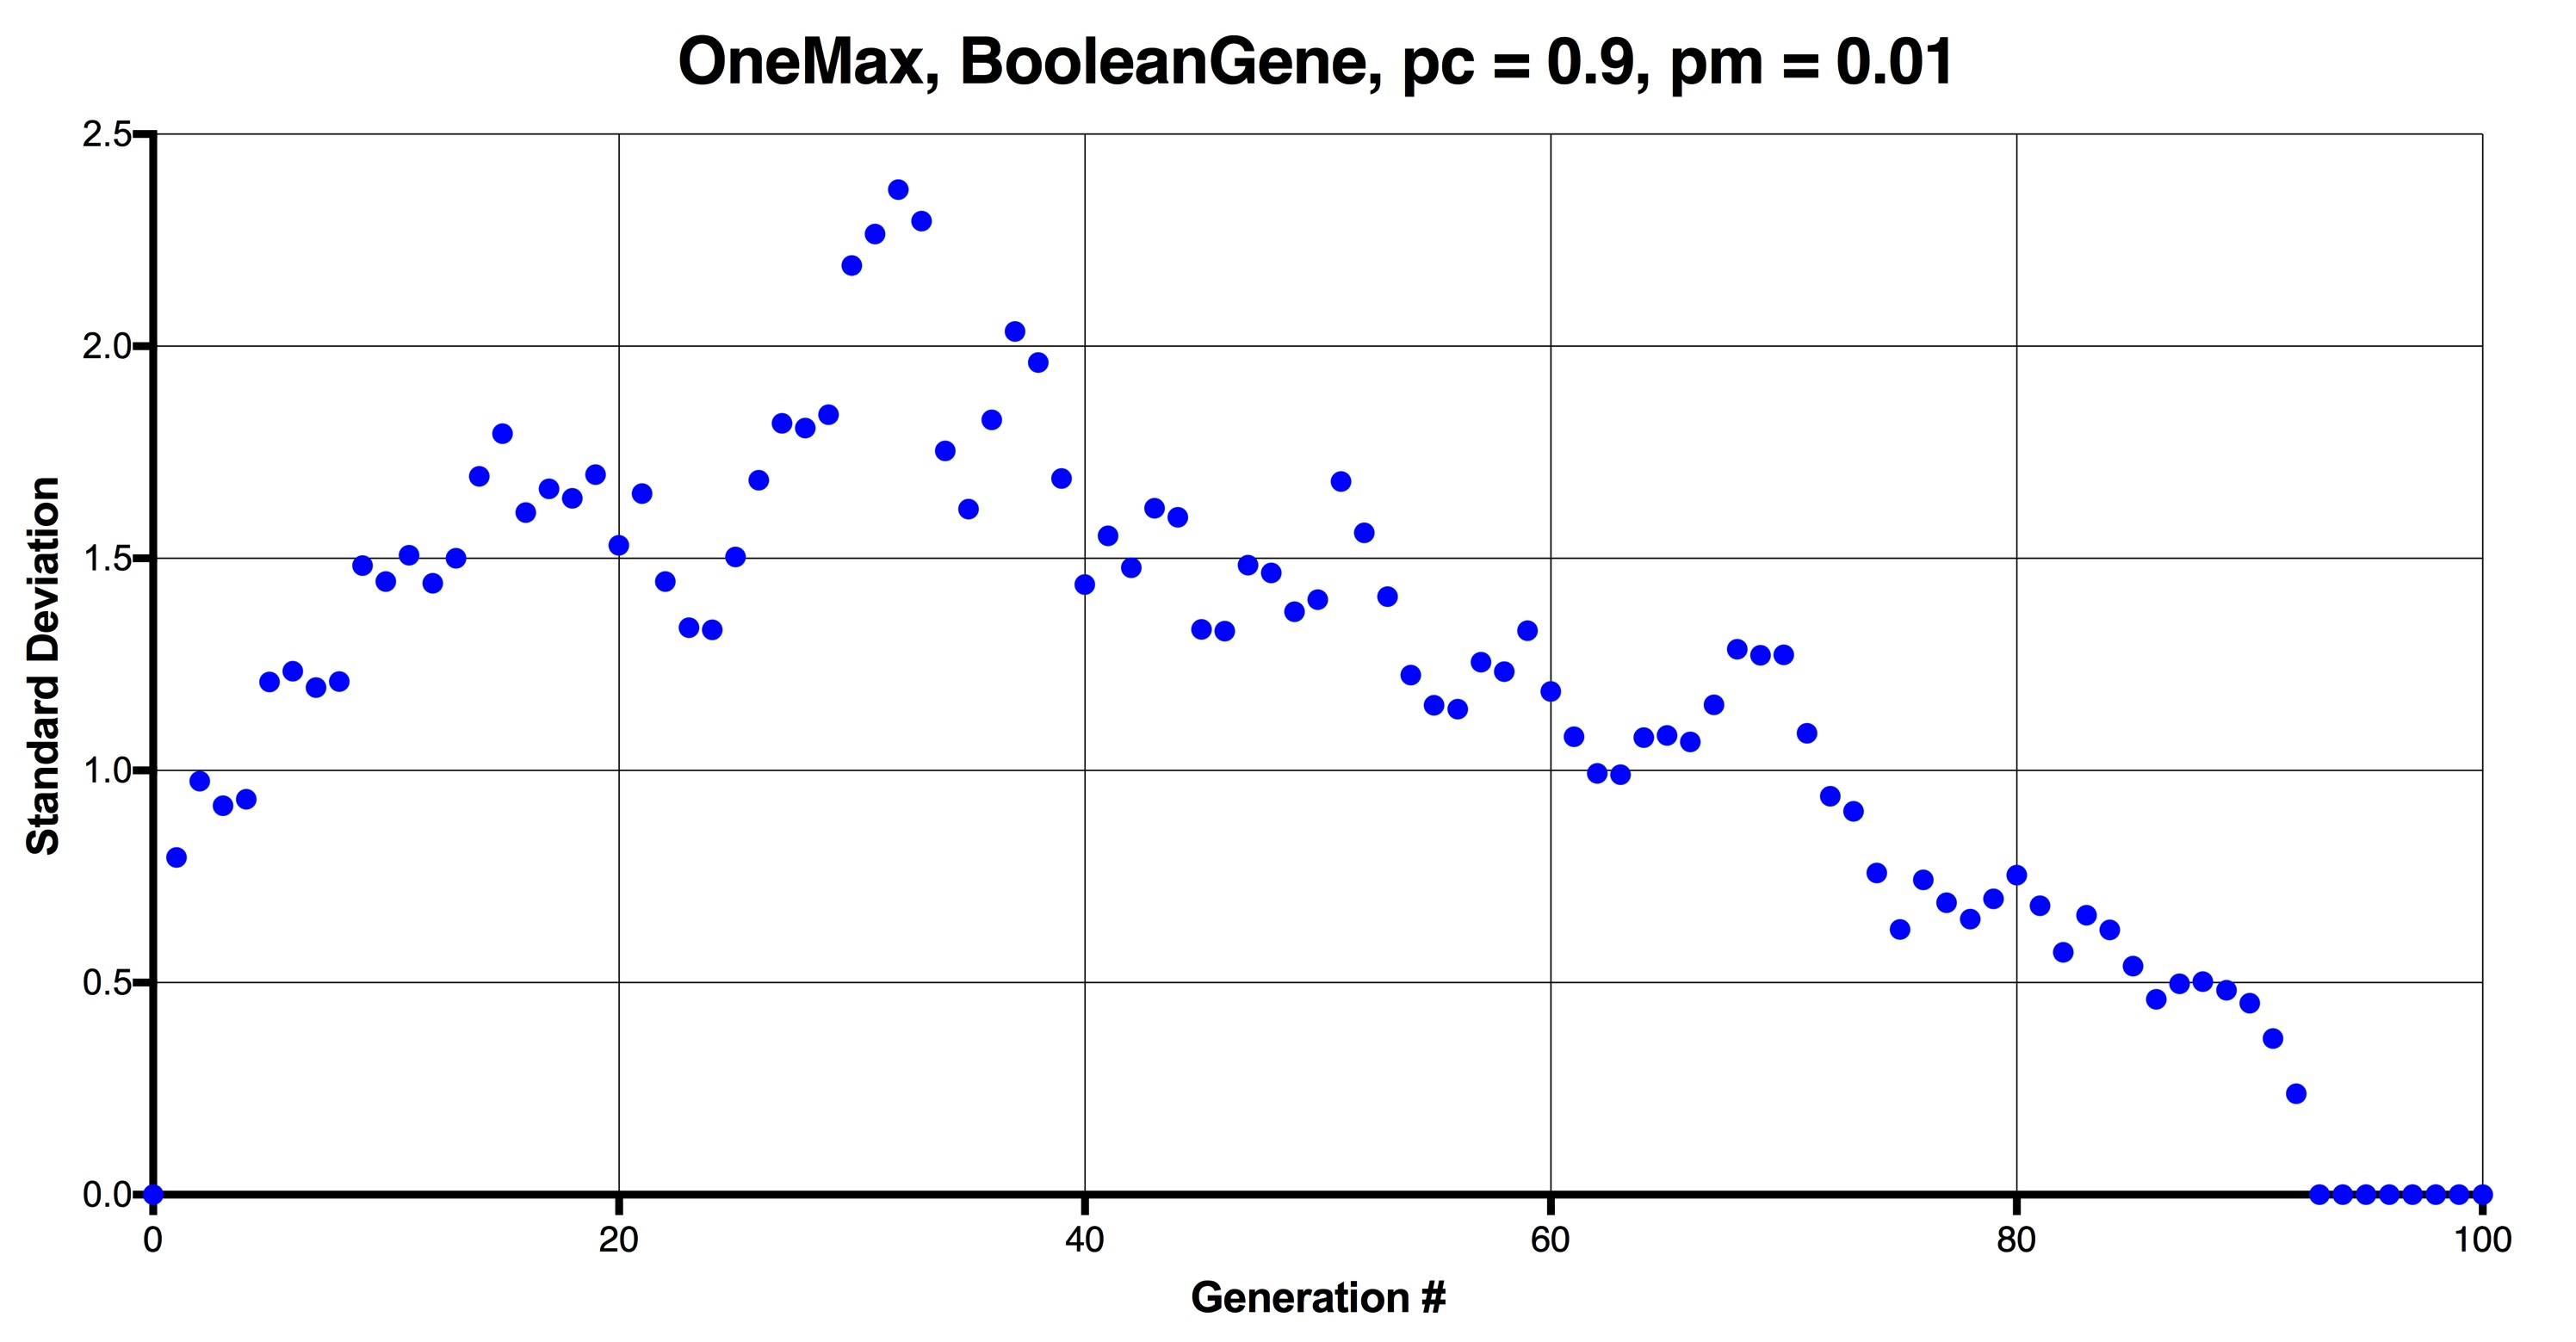
\includegraphics[width=1.0\textwidth]{onemax_boolean_std.jpg}
    \caption{Desvio padrão ao longo das gerações para o problema do OneMax Booleano ($p_c=0.9$, $p_m=0.01$).}
    \label{fig:onemax_boolean_std}
\end{figure}

\subsection{Caso Adaptativo}

\begin{figure}[ht!]
    \centering 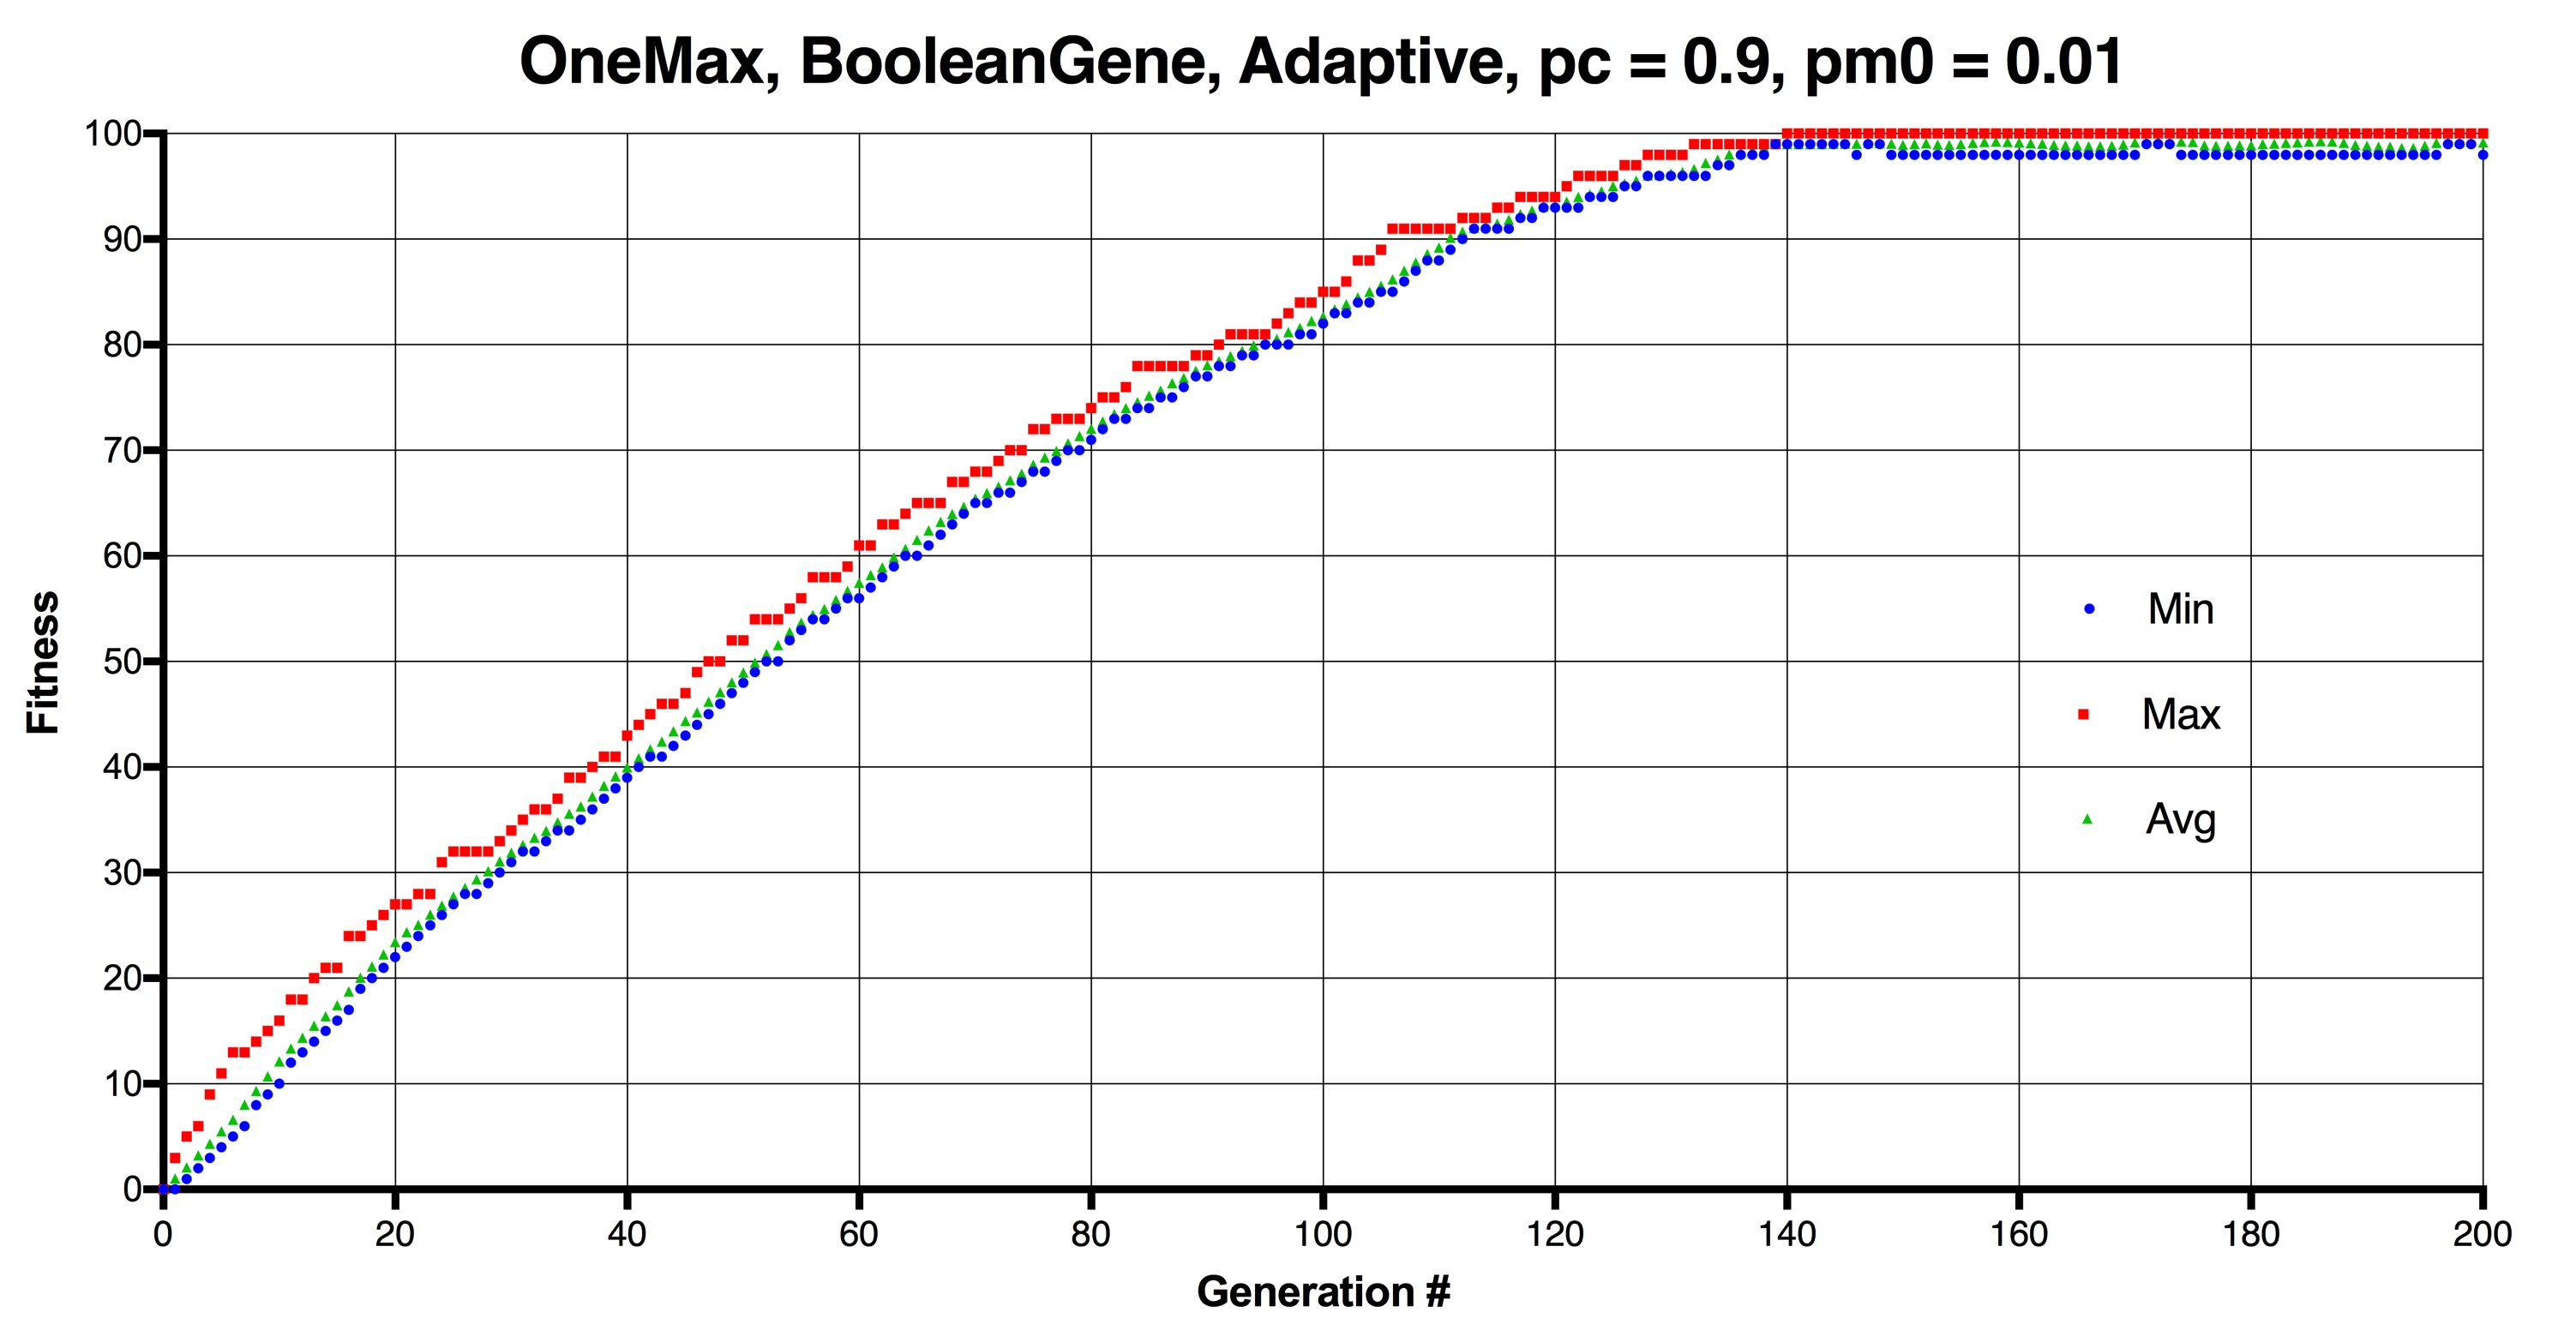
\includegraphics[width=1.0\textwidth]{onemax_boolean_adaptive.jpg}
    \caption{Evolução do fitness para o problema do OneMax Booleano Adaptativo mostrando mínimo, máximo e valor médio ($p_c=0.9$, $p_{m0}=0.01$).}
    \label{fig:onemax_boolean_adaptive}
\end{figure}

\begin{figure}[ht!]
    \centering 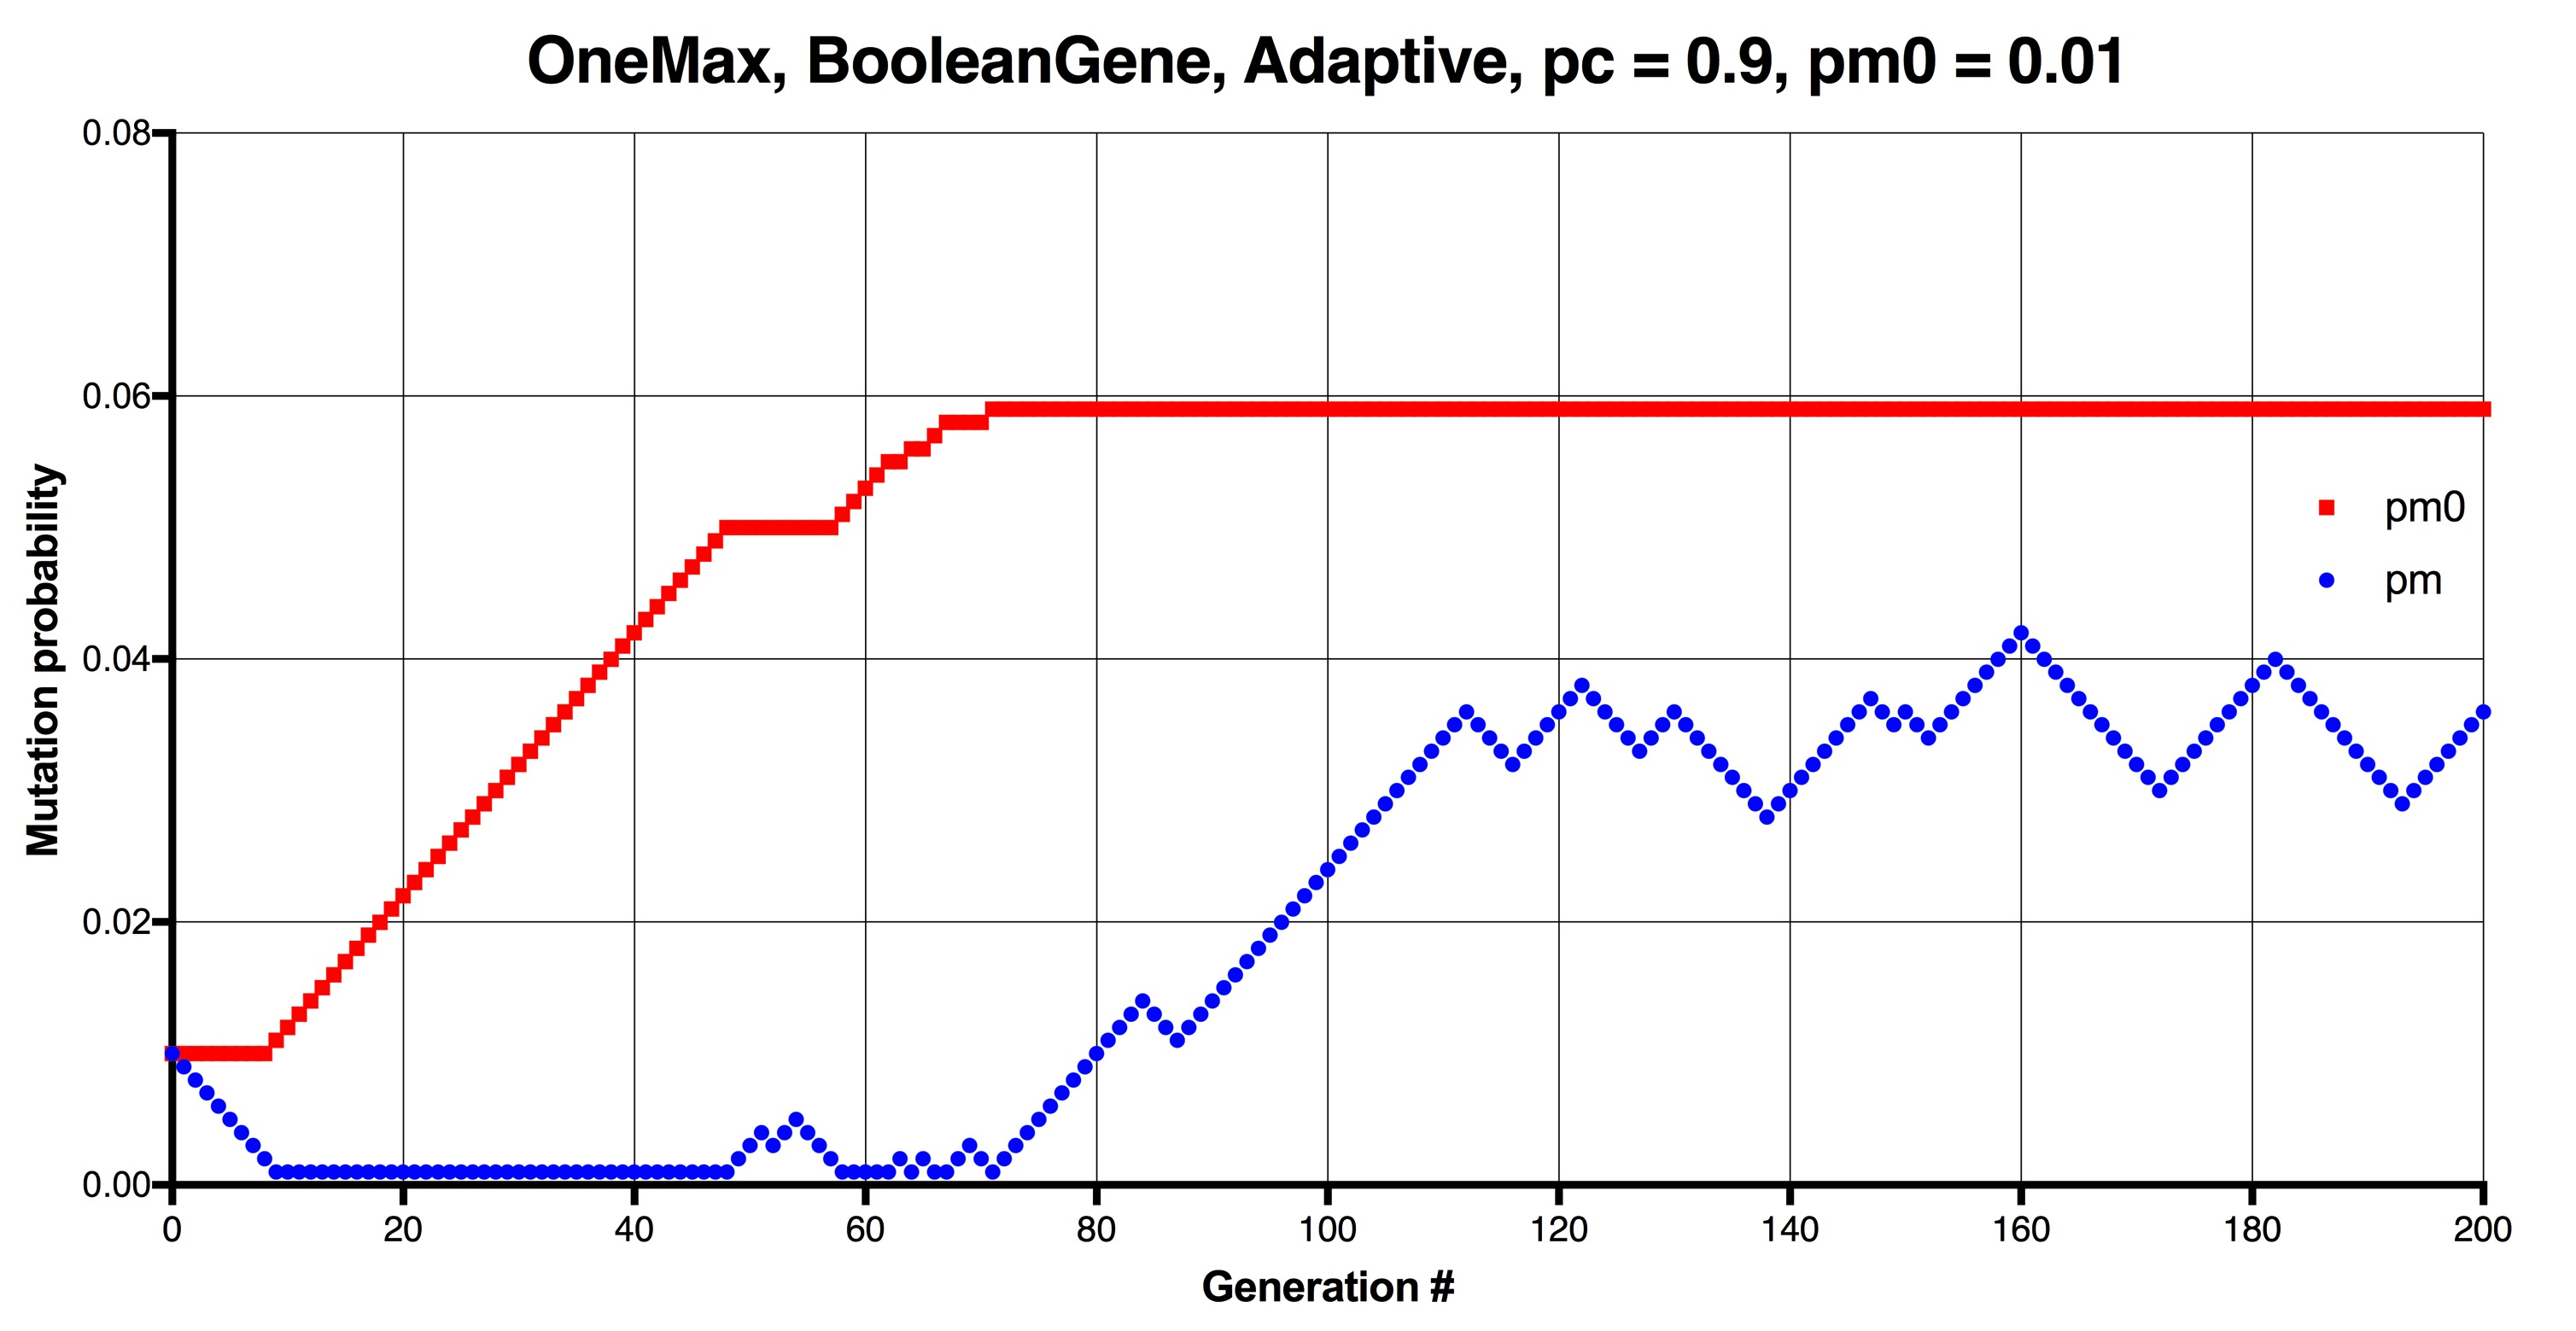
\includegraphics[width=1.0\textwidth]{onemax_boolean_adaptive_pm.jpg}
    \caption{Probabilidade de mutação ao longo das gerações para o problema do OneMax Booleano Adaptativo ($p_c=0.9$, $p_{m0}=0.01$).}
    \label{fig:onemax_boolean_adaptive_pm}
\end{figure}

\begin{figure}[ht!]
    \centering 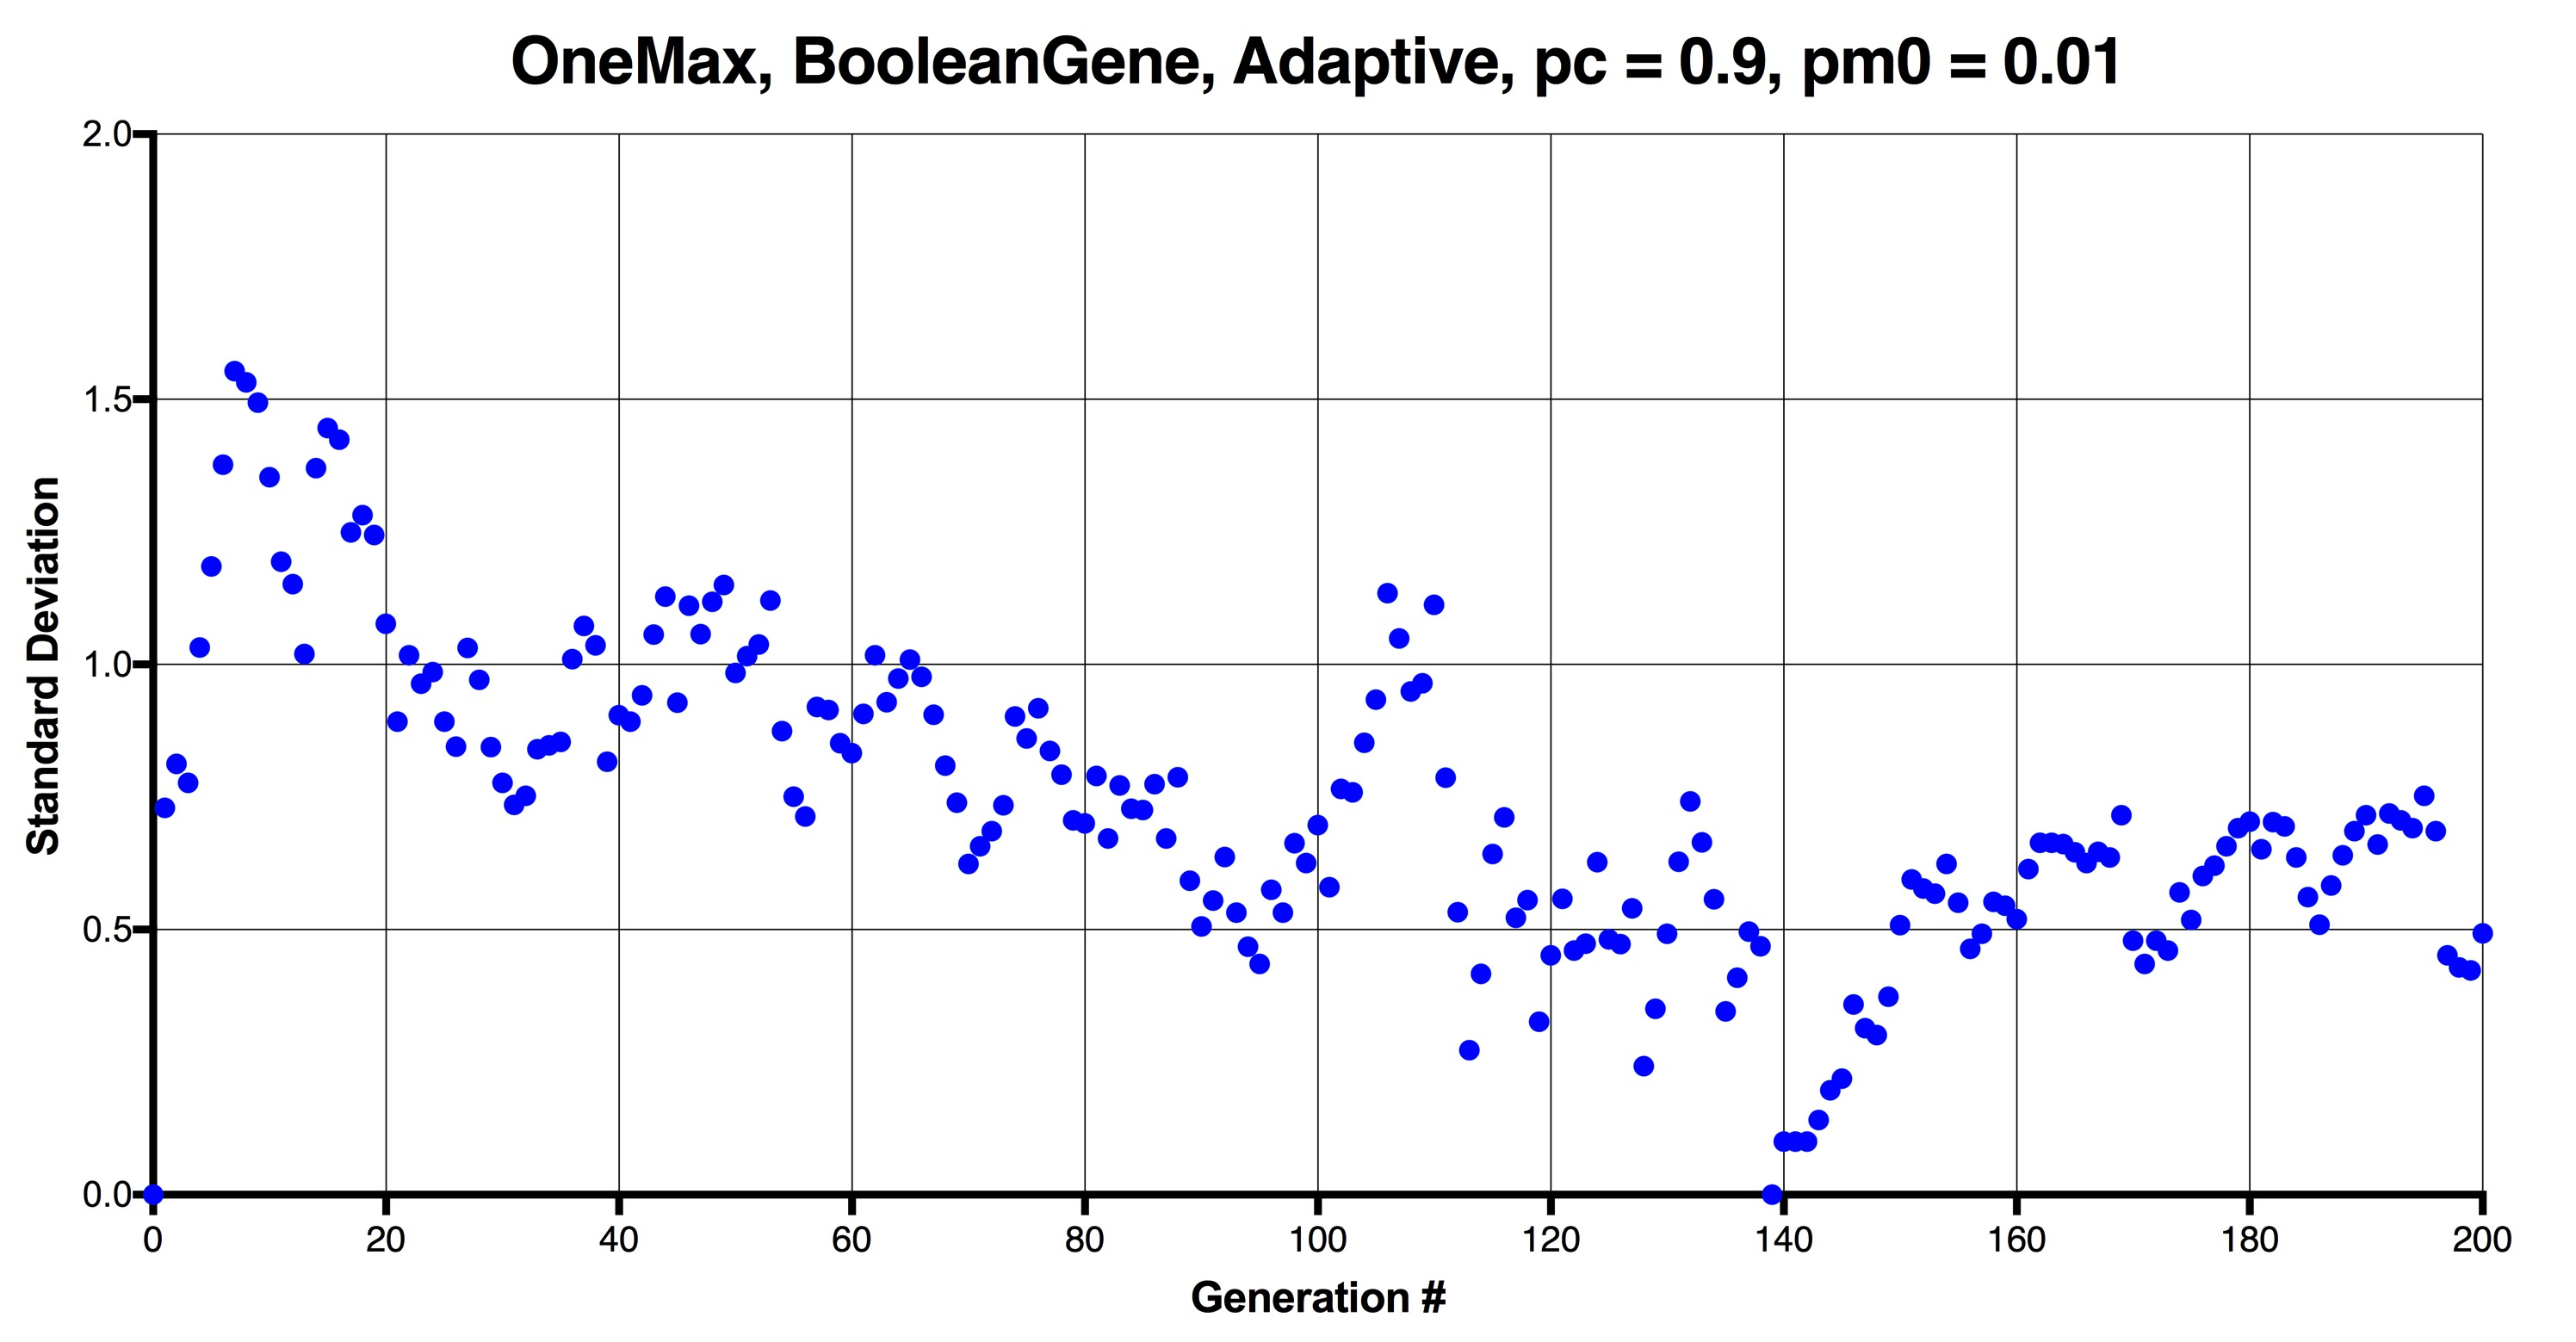
\includegraphics[width=1.0\textwidth]{onemax_boolean_adaptive_std.jpg}
    \caption{Desvio padrão ao longo das gerações para o problema do OneMax Booleano Adaptativo ($p_c=0.9$, $p_{m0}=0.01$).}
    \label{fig:onemax_boolean_adaptive_std}
\end{figure}

\section{OneMax Real}

Texto.

\begin{figure}[ht!]
    \centering 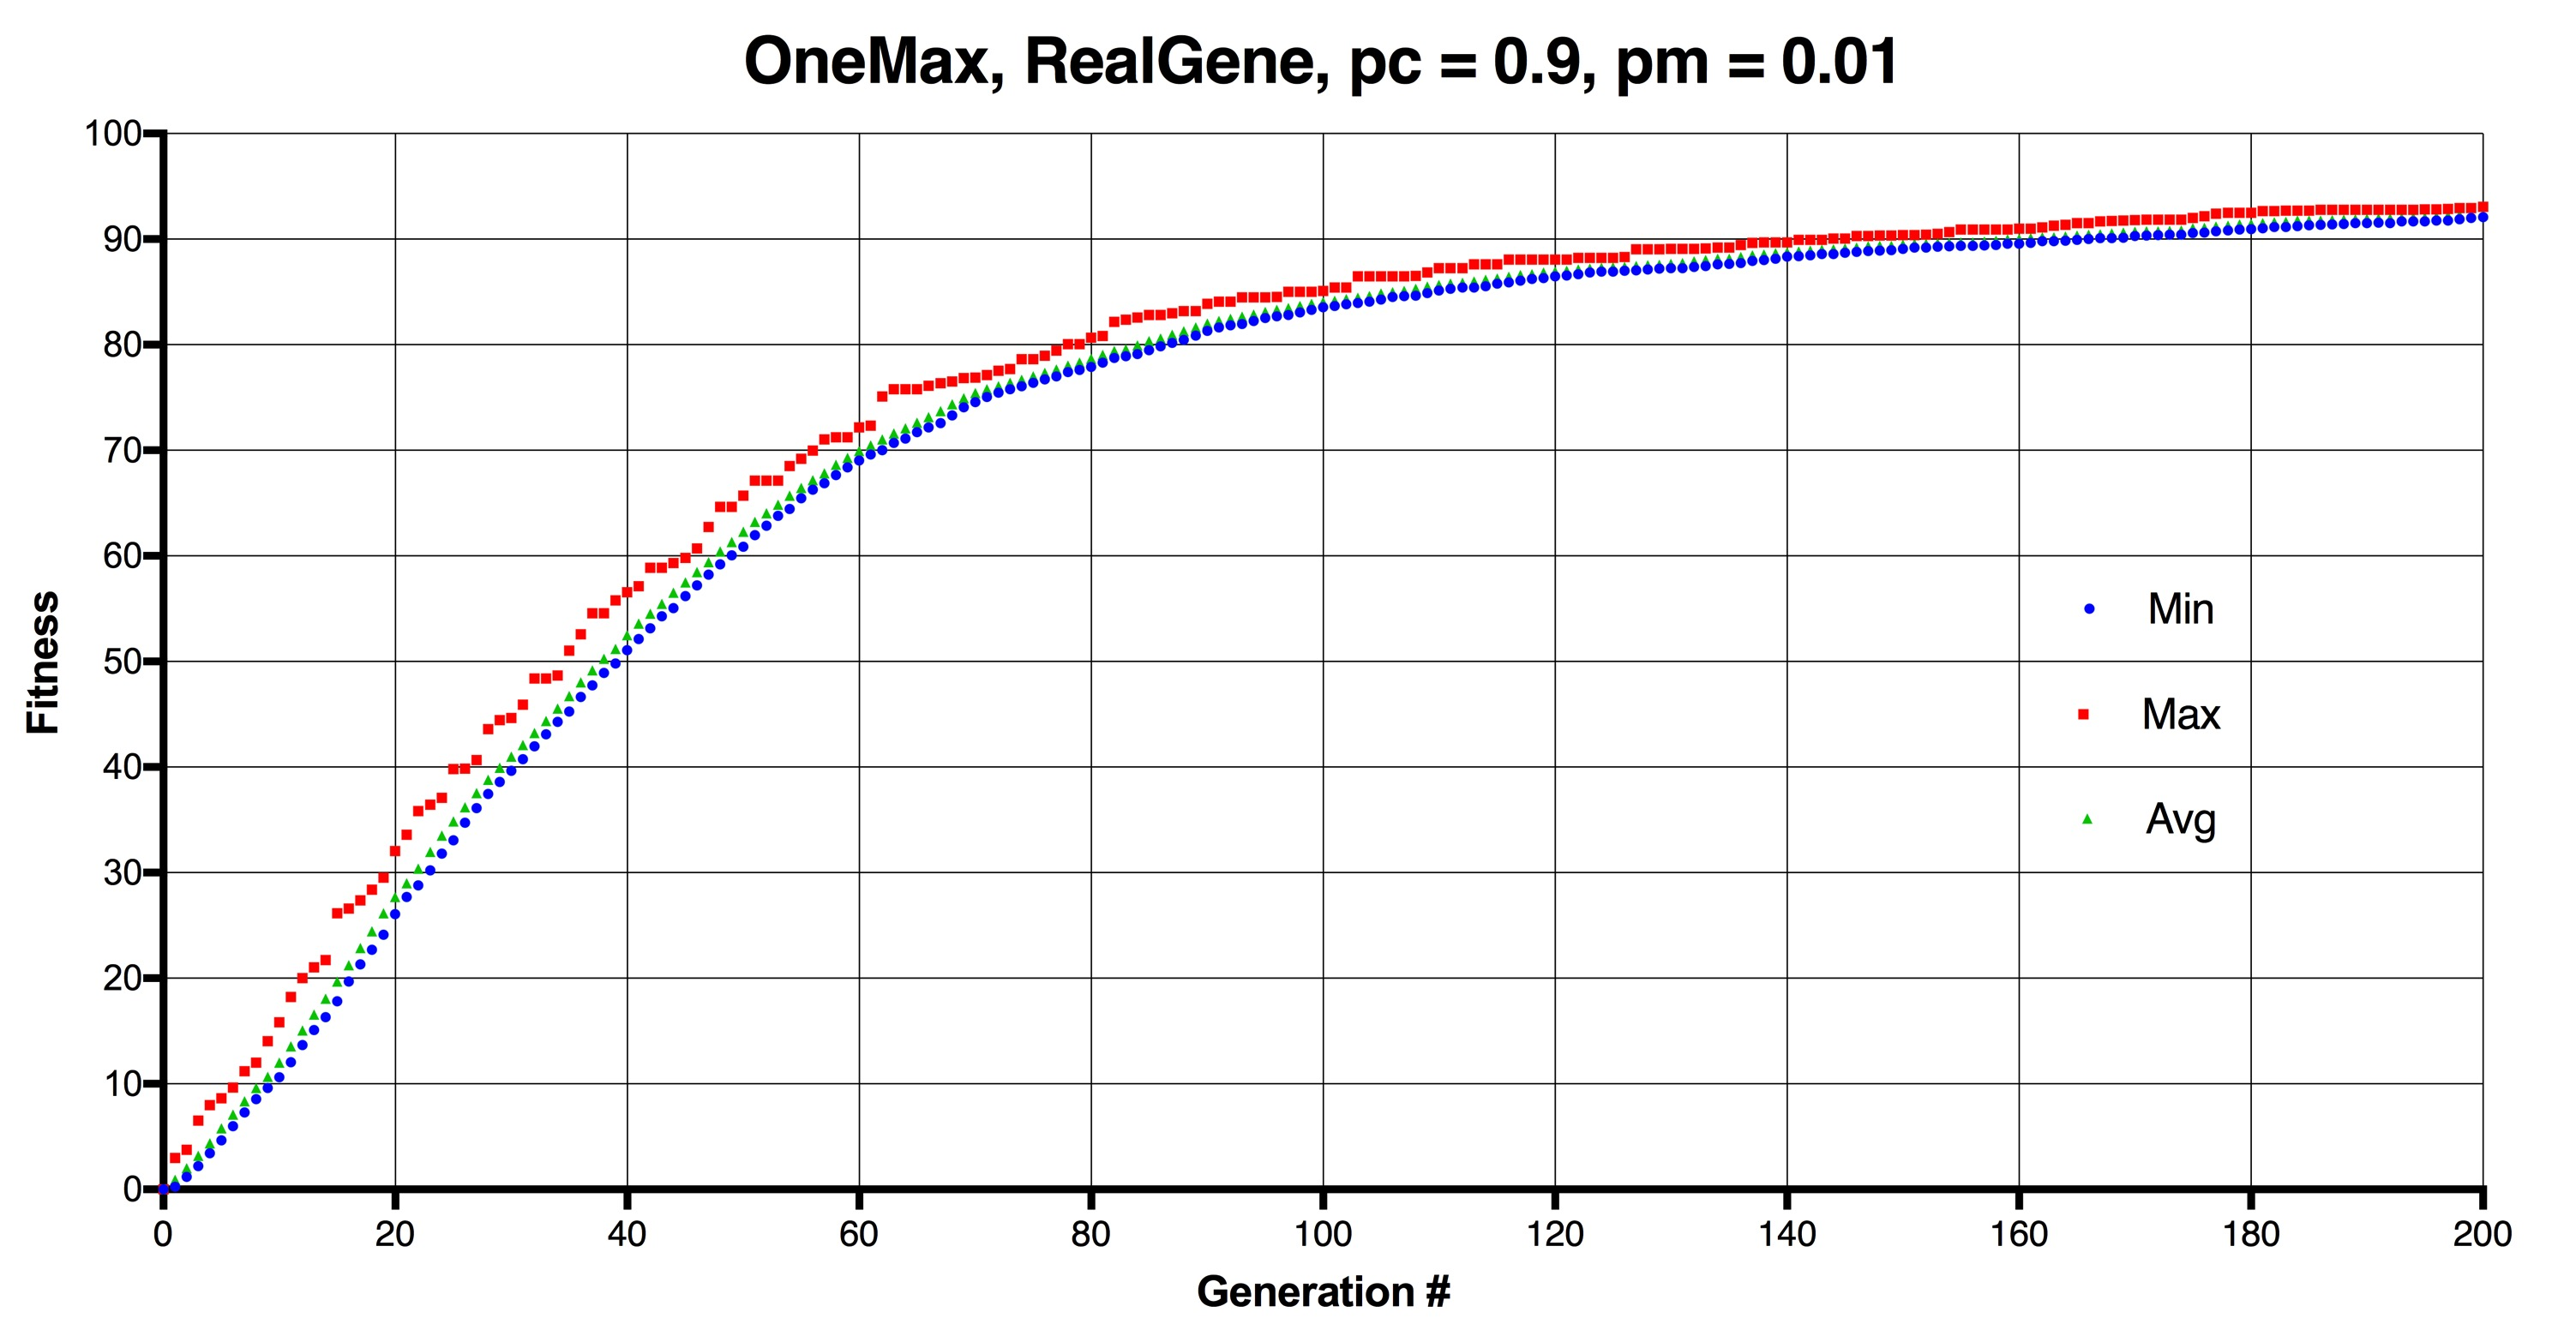
\includegraphics[width=1.0\textwidth]{onemax_real.jpg}
    \caption{Evolução do fitness para o problema do OneMax Real com mínimo, máximo e valor médio, com $p_c=0.9$ e $p_m=0.01$.}
    \label{fig:onemax_real}
\end{figure}

\begin{figure}[ht!]
    \centering 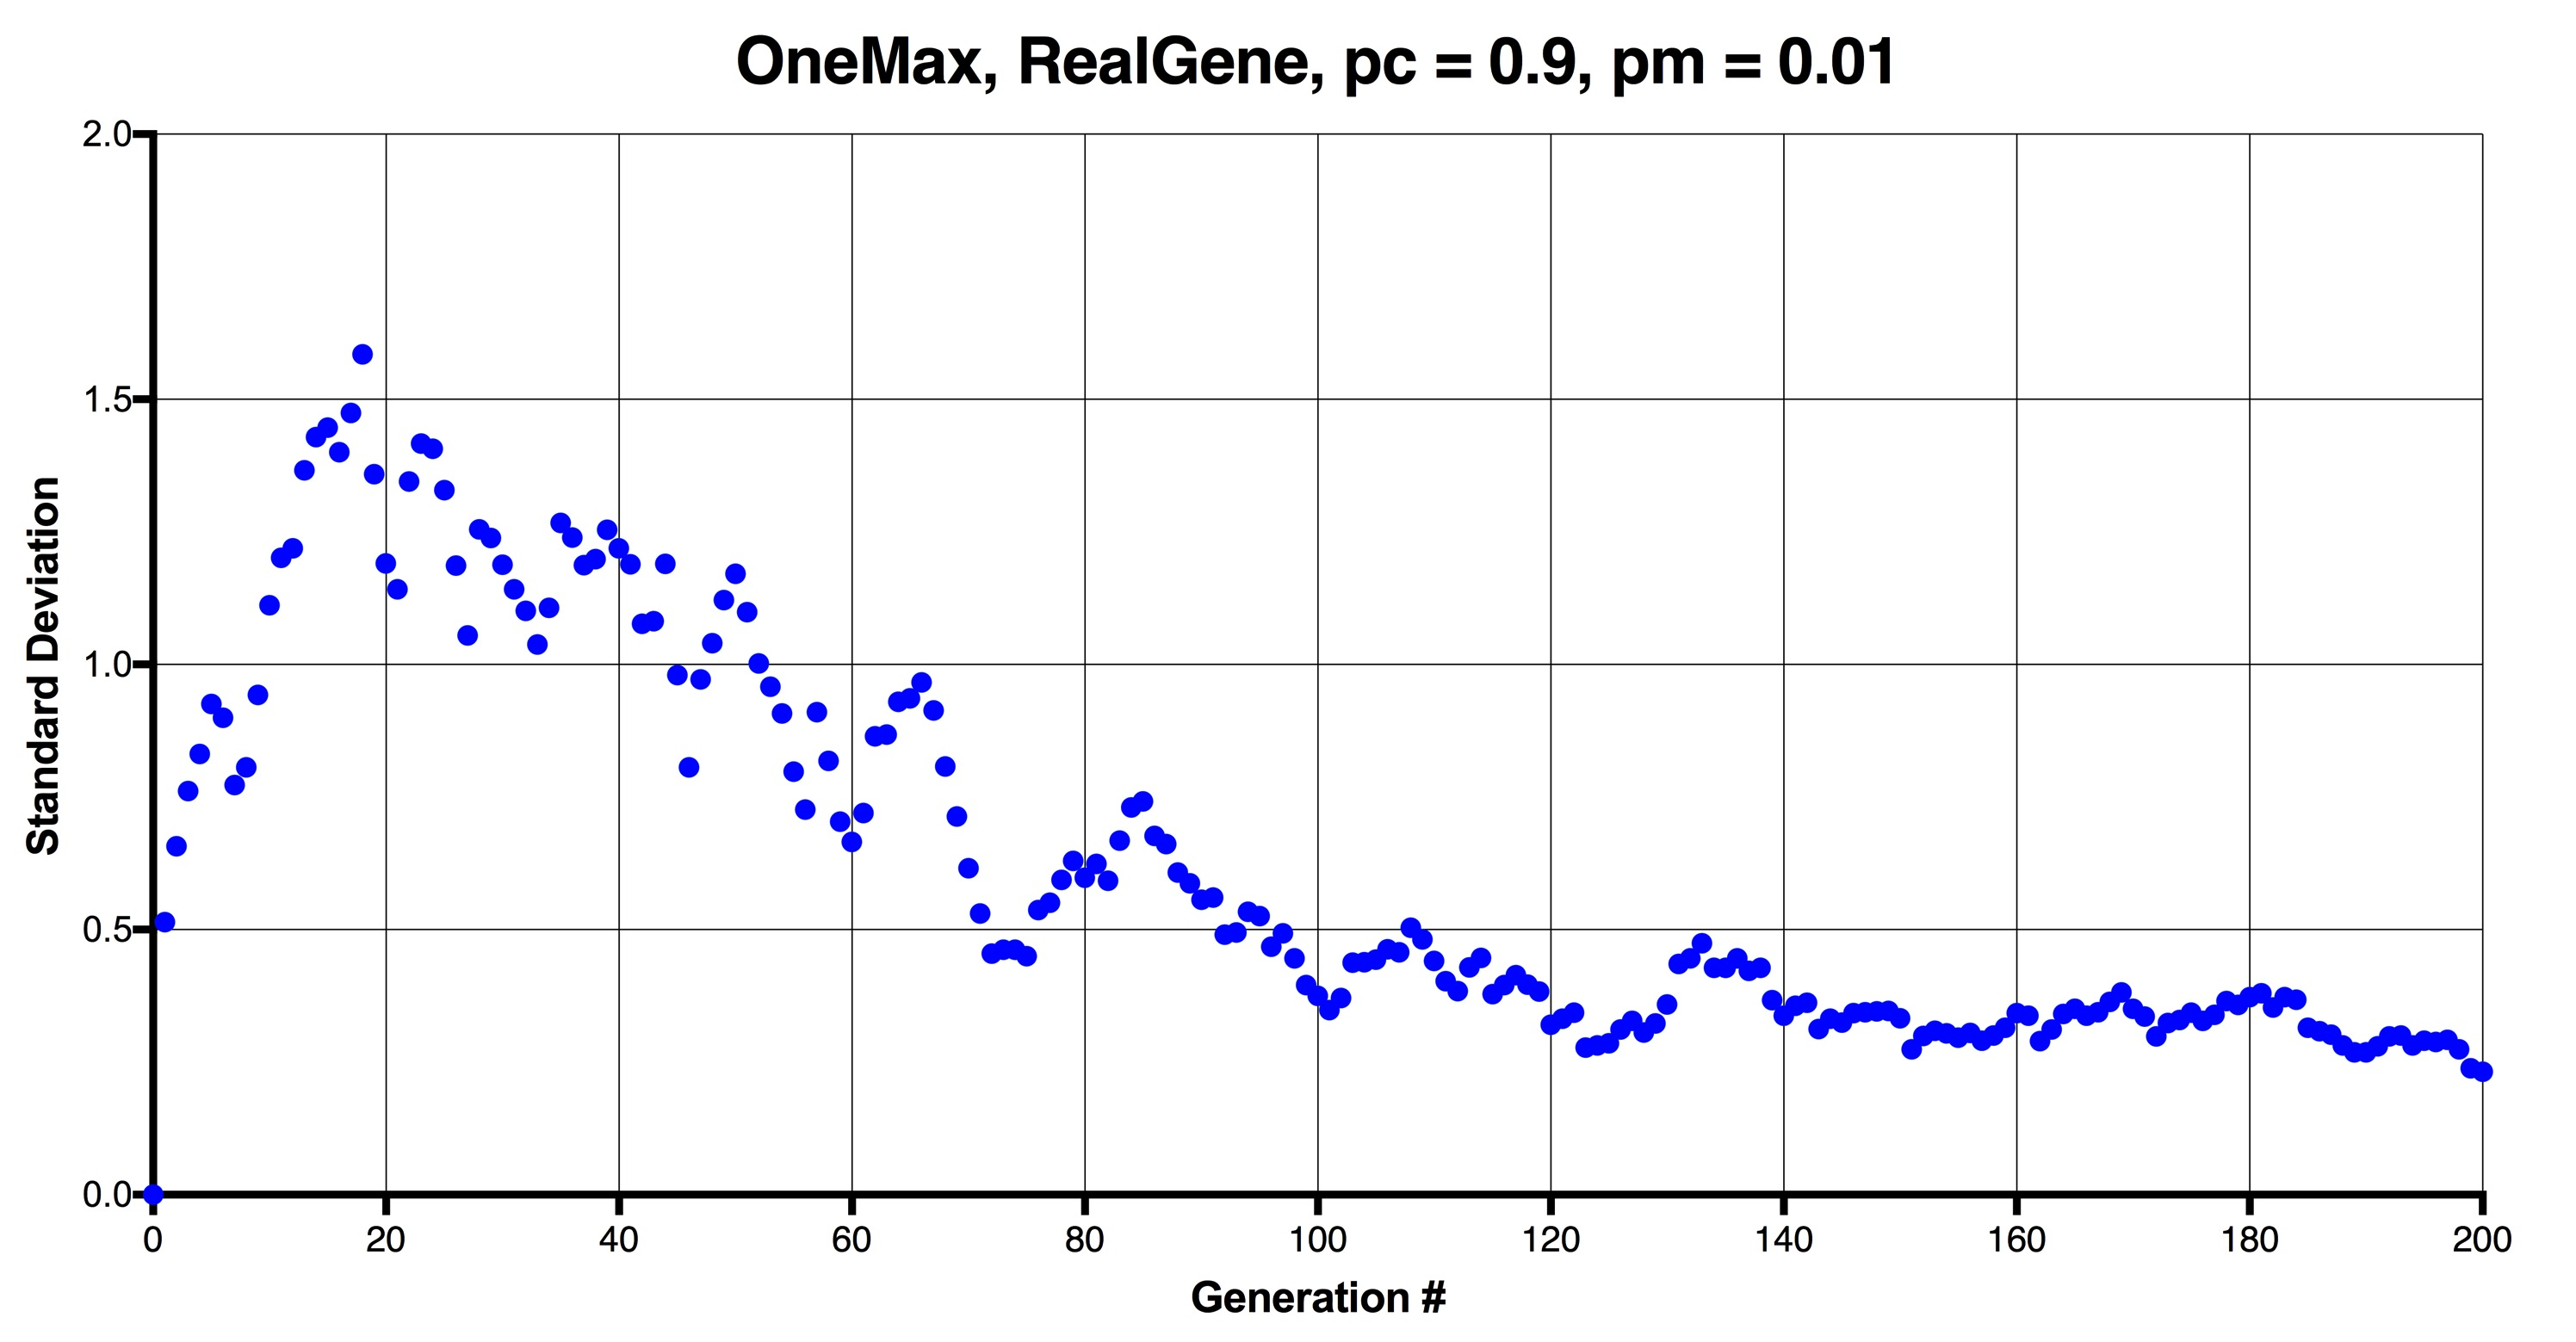
\includegraphics[width=1.0\textwidth]{onemax_real_std.jpg}
    \caption{Desvio padrão ao longo das gerações para o problema do OneMax Real, com $p_c=0.9$ e $p_m=0.01$.}
    \label{fig:onemax_real_std}
\end{figure}

\section{Caixeiro Viajante Adaptado}

Texto.

\begin{lstlisting}[float, floatplacement=H, caption={Mapa de cidades para o problema do Caixeiro Viajante Adaptado.}, label=lst:cidades]
[0, 633, 257, 91, 412, 150, 80, 134, 259, 505, 353, 324, 70, 211, 268, 246, 121],
[633, 0, 390, 661, 227, 488, 572, 530, 555, 289, 282, 638, 567, 466, 420, 745, 518],
[257, 390, 0, 228, 169, 112, 196, 154, 372, 262, 110, 437, 191, 74, 53, 472, 142],
[91, 661, 228, 0, 383, 120, 77, 105, 175, 476, 324, 240, 27, 182, 239, 237, 84],
[412, 227, 169, 383, 0, 267, 351, 309, 338, 196, 61, 421, 346, 243, 199, 528, 297],
[150, 488, 112, 120, 267, 0, 63, 34, 264, 360, 208, 329, 83, 105, 123, 364, 35],
[80, 572, 196, 77, 351, 63, 0, 29, 232, 444, 292, 297, 47, 150, 207, 332, 29],
[134, 530, 154, 105, 309, 34, 29, 0, 249, 402, 250, 314, 68, 108, 165, 349, 36],
[259, 555, 372, 175, 338, 264, 232, 249, 0, 495, 352, 95, 189, 326, 383, 202, 236],
[505, 289, 262, 476, 196, 360, 444, 402, 495, 0, 154, 578, 439, 336, 240, 685, 390],
[353, 282, 110, 324, 61, 208, 292, 250, 352, 154, 0, 435, 287, 184, 140, 542, 238],
[324, 638, 437, 240, 421, 329, 297, 314, 95, 578, 435, 0, 254, 391, 448, 157, 301],
[70, 567, 191, 27, 346, 83, 47, 68, 189, 439, 287, 254, 0, 145, 202, 289, 55],
[211, 466, 74, 182, 243, 105, 150, 108, 326, 336, 184, 391, 145, 0, 57, 426, 96],
[268, 420, 53, 239, 199, 123, 207, 165, 383, 240, 140, 448, 202, 57, 0, 483, 153],
[246, 745, 472, 237, 528, 364, 332, 349, 202, 685, 542, 157, 289, 426, 483, 0, 336],
[121, 518, 142, 84, 297, 35, 29, 36, 236, 390, 238, 301, 55, 96, 153, 336, 0]
\end{lstlisting}